\documentclass[11pt]{article}
\usepackage{MyTemplate}
\begin{document}
\thispagestyle{empty}
\settextfont[Scale=1.2]{B Nazanin}
\begin{center}

\includegraphics{logo}
\vskip 1cm
{\bf
دانشگاه صنعتی شریف\\ دانشکده مهندسی کامپیوتر\\ سمینار کارشناسی ارشد گرایش هوش مصنوعی\\
\vskip 1cm
عنوان:\\
دسته‌بندی ریزدانه‌ای  تصاویر‬\\
\lr{‫Fine-grained Image Classification}
\vskip 1cm
نگارش:\\
یاسر سوری\\
۹۲۲۰۴۷۴۴\\
\vskip 1cm
استاد راهنما:\\
دکتر شهره کسایی\\
\vskip 1cm
استاد ممتحن داخلی:\\
دکتر محمد تقی منظوری شلمانی\\

\vskip 3.5cm

}
شهریور ۹۳
\newpage
\end{center}




\settextfont[Scale=1]{XB Yas}
\setlatintextfont[Scale=0.95]{Times New Roman}
%\settextfont{B Nazanin}
%\settextfont{XB Yas}
%\settextfont{XB Kayhan}

{\bf {چکيده: }}
دسته‌بندی تصاویر ریزدانه‌ای عبارت است از دسته‌بندی تصاویر در حالتی که دسته‌های مورد نظر همگی زیر دسته‌ی یک دسته‌ی کلی‌تر هستند. برای مثال برای زیر دسته‌ی کلی پرندگان ما می‌توانیم گونه‌های مختلف پرندگان را در نظر بگیریم. در این حالت خاص مسئله دسته‌ها معمولاً از نظر ظاهری بسیار به یکدیگر شبیه هستند به گونه‌ای که افراد غیر متخصص نمی‌توانند دسته‌ها را از یکدیگر تمایز دهند. در چنین شرایطی راه حل‌های ارائه شده برای مسئله دسته‌بندی تصاویر معمولی اکثراً نتایج خوبی کسب نمی‌کنند. لذا ارائه روش‌هایی جدید برای حل این مسئله لازم است.
در این گزارش ابتدا به مرور روش‌های مهم در دسته‌بندی تصاویر معمولی و سپس به مرور روش‌های ارائه شده برای دسته‌بندی تصاویر ریزدانه‌ای می‌پردازیم. سپس روش انتخاب شده و دلایل انتخاب آن را بررسی می‌کنیم.
% تعریف مختصر راه حل
% در این گزارش چه مواردی بیان خواهد شد و چه نتیجه‌ای گرفته خواهد شد.


{\bf  { واژه‌های کلیدی: }}
بینایی کامپیوتری، بازشناسی شیء، دسته‌بندی تصاویر، بازشناسی ریزدانه‌ای، دسته‌بندی تصاویر ریزدانه‌ای.

\setlength{\parindent}{0.25in} %The indent of the paragraph first line

\section{مقدمه}\label{intro}
% تعریف مسئله
در دسته‌بندی تصویر 
\footnote{\lr{Image classification}}
هر تصویر با توجه به محتوایش دسته‌بندی می‌شود. برای مثال آیا تصویر شامل شی‌ء خودرو هست یا خیر. معمولاً در بینایی کامپیوتری مسئله بدین صورت است که تعدادی دسته مشخص را در نظر می‌گیریم (مثلاً انسان، خودرو، ساختمان، تلویزیون، صندلی، اسب و ...) سپس طبق چارچوب معمول یادگیری ماشین، توسط تعدادی تصویر شامل یکی از دسته‌ها (نمونه‌های مثبت) و تعدادی تصویر بدون شی‌ای از آن دسته (نمونه‌های منفی) یادگیری برای آن دسته انجام می‌شود. در نهایت پس از یادگیری تمام دسته‌ها در مواجهه با تصویر جدید لازم است تشخیص دهیم که آیا شی‌ای از هر کدام از آن دسته‌های مورد بررسی در تصویر وجود دارد یا خیر.
برای نمونه به شکل
\ref{fig:intro:img_class_data}
توجه کنید. در این شکل داده‌های آموزشی و آزمایشی برای دسته‌بند دسته‌ی «صفحه کلید
\footnote{\lr{Computer - Keyboard}}
» از پایگاه داده
Caltech256 \cite{caltech256}
 نشان داده شده است.

\begin{figure}[b!]
	\centering
	\begin{subfigure}[h]{0.5\textwidth}
		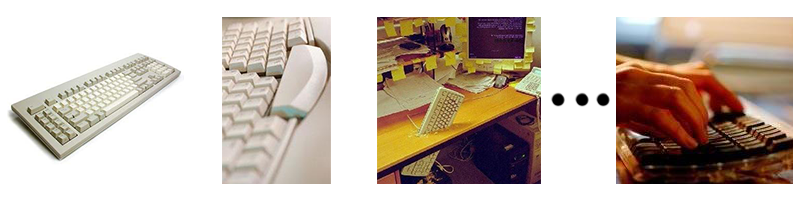
\includegraphics[width=\textwidth]{keyboard_positive}
		\caption{نمونه‌های مثبت، شامل شی‌ء صفحه کلید}
		\label{fig:intro:img_class_data:train_pos}
	\end{subfigure}
	\begin{subfigure}[h]{0.5\textwidth}
		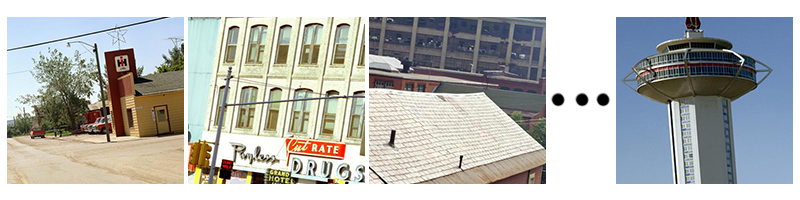
\includegraphics[width=\textwidth]{keyboard_negative}
		\caption{نمونه‌های منفی، بدون شی‌ء صفحه کلید}
		\label{fig:intro:img_class_data:train_neg}
	\end{subfigure}
	\begin{subfigure}[h]{0.5\textwidth}
		\centering
		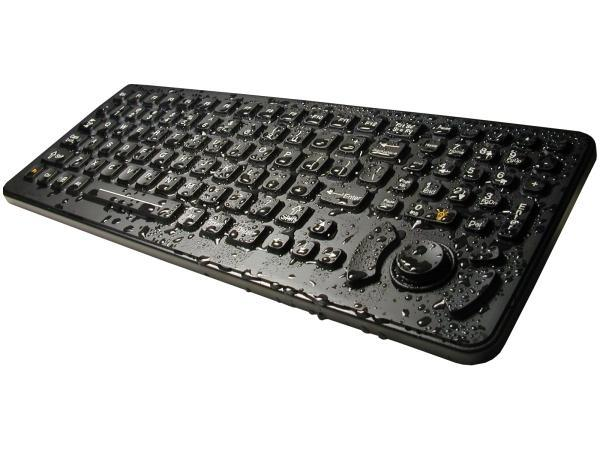
\includegraphics[width=0.5\textwidth]{keyboard_q}
		\caption{تصویر جدید آزمایش}
		\label{fig:intro:img_class_data:query}
	\end{subfigure}
 
	\caption{نمونه‌ای از تصاویر آموزشی و آزمایشی سامانه دسته‌بند تصاویر برای دسته‌ی «صفحه کلید». انتخاب شده از پایگاه داده
Caltech256 \cite{caltech256}.
			سامانه لازم است با مشاهده نمونه‌های مثبت \ref{fig:intro:img_class_data:train_pos} و نمونه‌های منفی \ref{fig:intro:img_class_data:train_neg} یادگیری را انجام داده و بتواند پاسخ دهد که در تصویر جدید آزمایشی \ref{fig:intro:img_class_data:query} آیا صفحه کلید وجود دارد یا خیر. برای این نمونه پاسخ مثبت است.
			}
	\label{fig:intro:img_class_data}
\end{figure}
چالش‌های اصلی این مسئله تنوع زیاد اشیاء درون هر کدام از دسته‌ها، نحوه‌ی عکس برداری و وجود اشیاء دیگر در تصویر است که باعث ایجاد تصاویری با تنوع بالا می‌شود. مدل کردن این تنوع مربوط به اشیاء هر دسته باید همزمان با توانایی تمایز بین دسته‌های مختلف باشد. برای نمونه شکل
\ref{fig:intro:img_class_discrim}
تصویری از دو دسته مختلف مربوط به پایگاه داده
Imagenet \cite{imagenet}
را نمایش می‌دهد. مدل دسته‌بند باید توانایی تمایز بین این دو دسته شبیه به هم را داشته باشد.

\begin{figure}[t]
	\centering
	\begin{subfigure}[h]{0.35\textwidth}
		\centering
		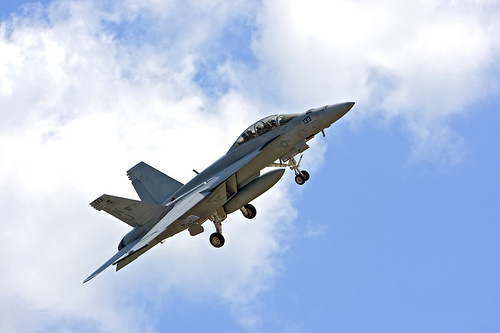
\includegraphics[height=4 cm]{fighter}
		\caption{هواپیمای جنگنده}
	\end{subfigure}
	\begin{subfigure}[h]{0.35\textwidth}
		\centering
		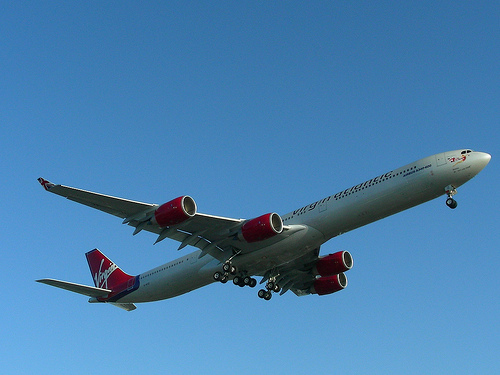
\includegraphics[height=4 cm]{airliner}
		\caption{هواپیمای مسافربری}
	\end{subfigure}
	\caption{نمونه‌ای از دو دسته‌ی متفاوت ولی شبیه به هم از پایگاه داده
Imagenet \cite{imagenet}.
مدل دسته‌بند علاوه بر توانایی مدل‌سازی تفاوت‌های داخل دسته‌ای، باید توانایی تمایز بین دسته‌های گاها شبیه به یکدیگر را داشته باشد.
}
	\label{fig:intro:img_class_discrim}
\end{figure}

اگر در دسته‌بندی تصویر، دسته‌های مورد بررسی زیر دسته‌ی
\footnote{\lr{Subclass}}
یک دسته‌ی کلی‌تر باشند(مانند گونه‌های مختلف پرندگان، مدل‌های مختلف خودروهای سواری و انواع مختلف هواپیماها)، آنگاه مسئله را «دسته‌بندی ریزدانه‌ای تصویر
\footnote{\lr{Fine-grained image classification}}»
می‌نامند. در دسته‌بندی ریزدانه‌ای تصویر معمولاً شباهت دسته‌ها به یکدیگر بسیار زیاد است به نحوی که افراد غیر متخصص نمی‌توانند به راحتی این دسته‌ها را بازشناسی نمایند. برای نمونه در شکل
\ref{fig:intro:terns}
چند گونه‌ی مختلف از پرستوی دریایی
\footnote{\lr{Tern}}
متعلق به پایگاه داده
CUB-200-2011 \cite{cub2002011}
نمایش داده شده است. همانگونه که می‌بینید با اینکه این نمونه‌ها به نحوی انتخاب شده‌اند که وضعیت مشابهی دارند، هنوز هم پیدا کردن ویژگی‌های تمایز دهنده بین گونه‌های مختلف کار بسیار سختی است و نیاز به تخصص دارد.

\begin{figure}[h]
	\centering
	\begin{subfigure}[h]{0.23\textwidth}
		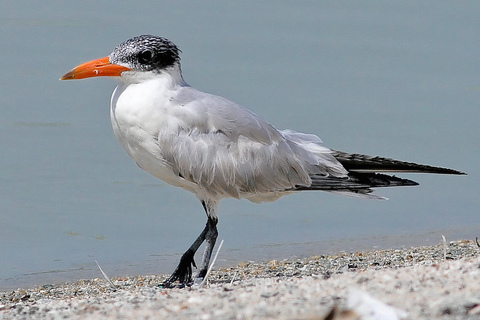
\includegraphics[height=2.5 cm]{Caspian_Tern}
		\caption{\lr{The Caspian tern}}
		\label{fig:intro:terns:1}
	\end{subfigure} 
	\begin{subfigure}[h]{0.23\textwidth}
		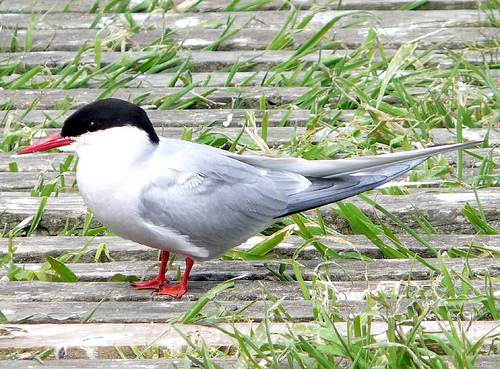
\includegraphics[height=2.5 cm]{Artic_Tern}
		\caption{\lr{The Artic tern}}
		\label{fig:intro:terns:2}
	\end{subfigure}
	\begin{subfigure}[h]{0.23\textwidth}
		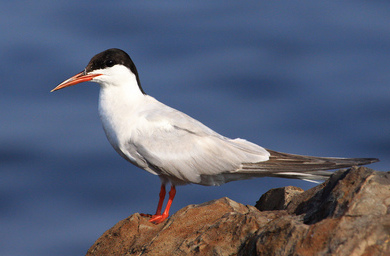
\includegraphics[height=2.5 cm]{Common_Tern}
		\caption{\lr{The common tern}}
		\label{fig:intro:terns:3}
	\end{subfigure}
	\begin{subfigure}[h]{0.23\textwidth}
		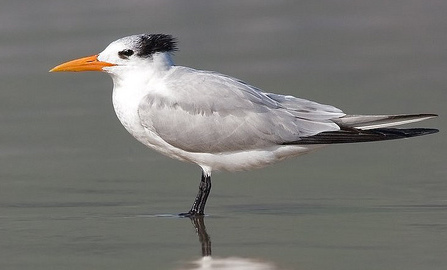
\includegraphics[height=2.5 cm]{Elegant_Tern}
		\caption{\lr{The elegent tern}}
		\label{fig:intro:terns:4}
	\end{subfigure}
	\caption{چهار گونه‌ی مختلف از پرستوهای دریایی متعلق به پایگاه داده
CUB-200-2011 \cite{cub2002011}.
شباهت بسیار زیاد بین دسته‌های مختلف کار را حتی برای افراد غیر متخصص بسیار سخت می‌کند.
}
	\label{fig:intro:terns}
\end{figure}

روش‌های دسته‌بندی تصویر معمولی در مسايل دسته‌بندی ریزدانه‌ای اکثراً موفق نیستند (به بخش فولان مراجعه شود). دلیل اصلی این عدم موفقیت وجود ویژگی‌های بسیار اندک و شدیداً محلی تمایزدهنده
\footnote{\lr{Discriminative}}
برای دسته‌های ریزدانه ایست. برای مثال دو گونه‌ی
\lr{elegent tern} در شکل \ref{fig:intro:terns:4}
و
\lr{common tern} در شکل \ref{fig:intro:terns:3}
فقط در رنگ پا و شکل تاج با یکدیگر تفاوت دارند و در سایر اجزا غیر قابل تمایز هستند. 

% کاربردها
% مراحل مختلف یک ردیاب عمومی


% اهمیت موضوع
مسئله مطرح بوده است.

% چالش‌ها
مسئله در حالت کلی بسیار مشکل است.


یک مسئله معکوس است. 

% دیتا ست و معیارهای مقایسه
برای مقایسه کارایی باشد.


\section{کارهای پیشین}\label{sec2}
به صورت یک مسئله تخمین حالت  سیستم پویا\footnote{\lr{Dynamic System}} در نظر گرفت.
\begin{equation}\label{equ:bayes}
p(X_t|\mathcal{I}_t) \propto  \underbrace{p(I_t|X_t)}_\text{درستنمایی}  \int{ \underbrace{p(X_t|X_{t-1})}_\text{مدل جابجایی} p(X_{t-1}|\mathcal{I}_{t-1}) dX_{t-1}}
\end{equation}

\linespread{1}
\small
\setlength{\parskip}{0pt}
\setlength{\parsep}{0pt}

\renewcommand{\bibname}{مراجع}
\begin{latin}
\bibliographystyle{IEEEtran}
%\bibliography{IEEEfull,ref}
\bibliography{IEEEabrv,ref}
\end{latin}



\section*{واژه‌نامه}
%\begin{LTR}
\begin{multicols}{3}
\theendnotes 
\end{multicols}
%\end{LTR}
\end{document}
